\section{力的几何性}\label{sec:04.06}

在\ref{sec:04.02}节中,当我们分析行星的运动时,只考虑太阳对行星的
引力;在分析月亮的运动时,只考虑地球对它的引力。实际上,
这样的分析是不严格的,因为月亮不仅受地球的引力作用,而且
也要受太阳的引力作用。计算一下就会发现,太阳对月亮的引力
与地球对月亮的引力相比,大小是差不多的,并不能作为小量加
% 139.jpg
以忽略。

为什么只考虑地球对月亮的作用,就能得到非常正确的结果
呢?原因在于太阳对月亮的作用效果与太阳对地球的作用效果是
完全一样的。这就是说,倘若地球和月亮之间没有作用,那么,
在太阳引力作用下,地球和月亮的轨道完全一样;在地球上来看,
月亮和地球的相对位置始终保持不变,好象根本不存在太阳的作
用一样。因此,当我们研究地球和月亮的相互关系时,可以不考
虑太阳的作用,而只考虑地球和月亮之间的相互作用。

“作用效果完全一样”,用数学语言来说,就是在下列方程
中,$ v_\text{月} $和$v_\text{地}$相等。
\begin{align}
  m _ { \text{月} } \frac { v _ { \text{月} } ^ { 2 } } { r } & = \frac { G m _ { \text{月} } M _ { \text{日} } } { r ^ { 2 } } \label{eqn:04.06.01} \\
  m _ { \text{地} } \frac { v _ { \text{地} } ^ { 2 } } { r } & = \frac { G m _ { \text{地} } M _ { \text{日} } } { r ^ { 2 } } \label{eqn:04.06.02}
\end{align}
其中$ m _ { \text{月} } , m _ { \text{地} } , v _ { \text{月} } , v _ { \text{地} } $分别是月球和地球的质量与速度;$ M _ { \text{日} } $是
太阳的质量;$ r $是地球到太阳的距离。应当注意,方程\eqref{eqn:04.06.01}和
方程 \eqref{eqn:04.06.02}两边质量的物理含义并不相同。方程左边的质量是牛
顿第二定律$ F = m a $中的质量,它的意义是力与加速度之比,是物
体惯性大小的度量,质量越大的物体,速度越难改变,所以称为
惯性质量。而方程右边的质量是牛顿引力定律$ F = m \alpha / r ^ { 2 } $中的质
量,它是质点感受外物引力大小的度量,质量越大,感受到外物
的引力越大,称为引力质量。为清楚起见,我们把式\eqref{eqn:04.06.01}、
\eqref{eqn:04.06.02}改写为
\begin{align}
  \left(m _ { \text{月} }\right) _ {\text{惯}}
  \frac { v _ { \text{月} } ^ 2 } { r } & = \frac { G \left(m _ { \text{月} }\right) _ {\text{引}} M _ { \text{日} } } { r ^ { 2 } }\label{eqn:04.06.03} \\
  \left(m _ { \text{地} }\right) _ {\text{惯}}
  \frac { v _ { \text{地} } ^ 2 } { r } & = \frac { G \left(m _ { \text{地} }\right) _ {\text{引}} M _ { \text{日} } } { r ^ { 2 } }\label{eqn:04.06.04}
\end{align}
其中下标“惯”表示惯性质量,“引”表示引力质量由式\eqref{eqn:04.06.03}
% 140.jpg
、\eqref{eqn:04.06.04}可知,要求$ v _ { \text{月}}=v _ { \text{地} } $,等价于
\begin{equation}\label{eqn:04.06.05}
  \frac { \left(m _ { \text{月} }\right) _ {\text{惯}} } { \left(m _ { \text{月} }\right) _ {\text{引}} } = \frac { \left(m _ { \text{地} }\right) _ {\text{惯}} } { \left(m _ { \text{地} }\right) _ {\text{引}} }
\end{equation}
式\eqref{eqn:04.06.05}就是我们在处理地月相互关系时可以忽略太阳作用的
根据。我们可以把上述的论证推广,得到对任何物体$ A $都有
\begin{equation}\label{eqn:04.06.06}
  \frac { \left(m _ { A }\right) _ {\text{惯}} } { \left(m _ { A }\right) _ {\text{引}} } = \frac { \left(m _ { \text{地} }\right) _ {\text{惯}} } { \left(m _ { \text{地} }\right) _ {\text{引}} }
\end{equation}
因此,任一物体的惯性质量与引力质量之比都应等于一普适常数,
即
\begin{equation}\label{eqn:04.06.07}
  \frac { m _ {\text{惯}} } { m _ {\text{引}} } = \text{普适常数}
\end{equation}
显然,只要单位选择适当,总可以使这个普适常数为1。

对于上述论断,在历史上曾多次用实验来检验。最著名的实
验是 E\"otv\"os 在1890年做的,他的仪器如图\ref{fig:04.05}所示。先调整扭秤
处于“自然”状态(即扭丝没有扭转),安放于图\ref{fig:04.05b}所示的位
置,然后把两个引力质量相等但材料不同的物体$ A, B $分别放置在
扭秤的两臂上\lhbrak 图\ref{fig:04.05a}\rhbrak 。因为$\left(m _ { A }\right) _ {\text{引}} = \left(m _ { B }\right) _ {\text{引}} $,所以$ A , B $受
到太阳的引力作用相等。如果$ A , B $的惯性质量不等,设$ \left(m _ { A }\right) _ {\text{惯}} > \left(m _ { B }\right) _ {\text{惯}} $,则当$ A , B $随地球绕太阳公转时,所受向心力不等,故
悬丝将产生一扭转,杆将处于如图\ref{fig:04.05c}所示的状态(图中$ C $点
为地球上的观察者)。12小时后,由于地球自转,地球上的观察
者$ C $将由靠近太阳的一侧,转到远离太阳的一侧。同上分析,杆
转到如图\ref{fig:04.05d}所示的状态。因此,对地球上的观察者$ C $来说,
他看到扭秤将有以$ 24 $小时为周期的摆动。

E\"otv\"os 用一些不同材料的物体悬在扭秤上做过多次实验,
在实验误差范围内观察不到杆发生摆动。从而得出结论:在精确
度为$ 1 0 ^ { - 8 } $的范围内,各种物体的惯性质量与其引力质量的比是一
常数。1964年, Dicke 把实验精度提高到$ 1 0 ^ { - 1 0 } $, 1971 年,又提高
% 141.jpg
到$ 1 0 ^ { - 1 1 } $。E\"otv\"os 实验是到目前为止精度最高的著名物理实验之一。
\begin{figure}[t]
  \centering
  \subfigure[\label{fig:04.05a}]{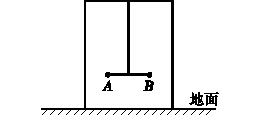
\includegraphics{figure/fig04.05a}} \qquad
  \subfigure[\label{fig:04.05b}]{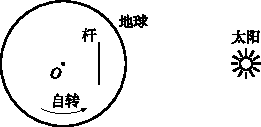
\includegraphics{figure/fig04.05b}}
  \subfigure[\label{fig:04.05c}]{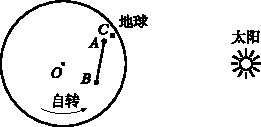
\includegraphics{figure/fig04.05c}} \qquad
  \subfigure[\label{fig:04.05d}]{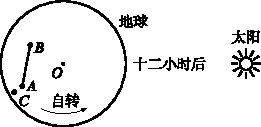
\includegraphics{figure/fig04.05d}}
  \caption{E\"otv\"os 实验示意图}
  \label{fig:04.05}
  \vspace{-0.8em}
\end{figure}

其实,在 E\"otv\"os 之前,就有人做过这类实验。伽利略的比
萨斜塔实验以及斜面实验,证明了不同物体的自由落体运动是一
样的,与物体的质料无关。牛顿也设计过验证惯性质量与引力质
量的比为普适常数的实验。我们很容易推导出单摆周期$ T $为
\begin{equation*}
  T = 2 \uppi \sqrt{\frac { m _ {\text{惯}} l } { m _ {\text{引}} g }}
\end{equation*}
其中$ m _ {\text{惯}} $及$ m _ {\text{引}} $分别是摆锤的惯性质量及引力质量;$ l $是摆长。牛
顿用不同材料作摆锤,做过多次实验。如果惯性质量和引力质量
的比不是普适常数,将会反映在摆周期的变化上。但是牛顿发现,
在所有这些情况下,摆的周期都相同。当然,这实验的精度远不
如E\"otv\"os的实验精度。

存在普适常数式\eqref{eqn:04.06.07}是引力所具有的一个基本性质,即引
力的几何性。下面我们来讨论引力几何性的含意。

我们知道,开普勒第三定律说,任何行星的运动周期的平方
% 142.jpg
与其椭圆轨道半长轴的三次方成正比。这是描写行星运动规律的
定律,它只涉及度量行星运动的时间量和度量轨道的空间量,即
仅仅涉及几何量,而并没有涉及到行星本身的任何物性。运动学
只涉及几何量,动力学则应当涉及物性。因为动力学是研究物体
\begin{wrapfigure}[10]{r}{15em}
  \centering
  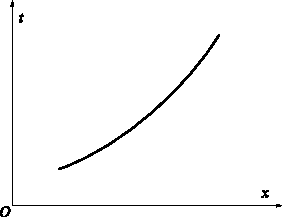
\includegraphics{figure/fig04.06}
  \caption{一维运动的时-空图}
  \label{fig:04.06}
\end{wrapfigure}
之间的相互作用力如何使物体产生运动,而相互作用力
一般是和物性有关的。但开普勒第三定律中却不含物
性,这就是引力几何性的一个反映。

对于质点运动,我们可以用时-空图来表示,图\ref{fig:04.06}
是一维运动的时-空图。如果已知质点轨道方程为
\begin{equation*}
  x = x \left( t \right)
\end{equation*}
我们可在时-空图上绘出相应的曲线。从曲线上,可求得在任何时
\begin{wrapfigure}[10]{l}{16em}
  \vspace{-1em}
  \centering
  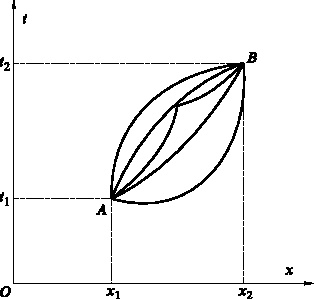
\includegraphics{figure/fig04.07}
  \caption{$ A $,$ B $之间可能的运动}
  \label{fig:04.07}
\end{wrapfigure}
刻质点的位置、速度等。因此,它能完全表达质点的运动。

从运动学来说,如果只告诉我们质点在$ t_1 $时位于
$ x_1 $,在$ t_2 $时运动到$ x_2 $,那么这中间可以有无穷多种可能
的选择,即可写出无穷多种满足上述要求的运动方程。
反映在时-空图上(图\ref{fig:04.07})就是,每一种选择对应一条过
$ A $,$ B $点的曲线,即可作无
% 143.jpg
穷多种时空曲线连接$ A $,$ B $两点。

现在我们来讨论质点在地面附近重力场中沿竖直线运动的一
维情形。如果质点受重力作用,而且仅受重力作用,且$ t _ { 1 } $时刻在
$ x _ { 1 } , t _ { 2 } $时刻运动到$ x _ { 2 } $,那么它的轨道方程是
\begin{equation*}
  x = x _ { 0 } + v _ { 0 } t - \frac { 1 } { 2 } g t ^ { 2 }
\end{equation*}
而且其中的常数$ x _ { 0 } $和$ v _ { 0 } $将由$ \left( t _ { 1 }, x _ { 1 } \right) , \left( t _ { 2 } , x _ { 2 } \right) $唯一地确定。这就
是说,在时-空图上只能有一条连接$ A , B $的时空曲线,而绝不允
许有其他的任何选择,对任何质料的物体均如此(即在连接$ A , B $
的时空曲线的方程中,没有标志物性的因子或系数;对各种质料
而言,曲线是唯一的)这就是重力的几何性

\begin{wrapfigure}[11]{r}{15em}
  \centering
  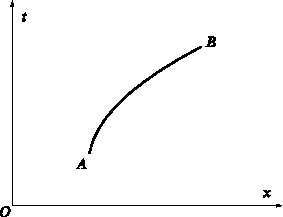
\includegraphics{figure/fig04.08}
  \caption{$ A $,$ B $之间唯一可实现的时空曲线}
  \label{fig:04.08}
\end{wrapfigure}
对于引力控制的运动,也与重力有相同的性质。对
任何质料的物体,若给定初始和终了的时空点,则引力
决定了物体在时-空图上的唯一可实现的曲线,即决定
了运动物体的时间和空间的几何性质。引力的这种几何
性是引力的最大特点,其他力(例如电磁力等)没有这种
性质。

从动力学方程很容易看到这个特点,在万有引力情况,有
\begin{equation*}
  m a = \frac { G m M } { r ^ { 2 } }
\end{equation*}
可得
\begin{equation*}
  a = \frac { G M } { r ^ { 2 } }
\end{equation*}
因为引力质量和惯性质量相同,故二者从方程中消去了。这样,
% 144.jpg
\clearpage\noindent
在上述方程中就不含有运动物体本身的物性,而只是一种几何的
关系式。但在其他力的情况,没有这个性质。
